\subsection{DTW with Global Invariances}
\label{sec:dtw_gi}

In this work, we address the problem of comparing time series while taking
into account both feature space transformation and temporal variability.
The proposed framework combines a latent global transformation of the feature
space with the widely used Dynamic Time Warping (DTW).
This work is available as a preprint~\cite{vayer2020time}.%
\footnote{\label{fn:titouan}This work is part of Titouan Vayer's PhD thesis.
We are co-supervising Titouan together with Laetitia Chapel and Nicolas Courty.}

\subsubsection{Definition}

Let $\mathbf{x}$ and $\mathbf{x^\prime}$ be two time series of respective
lengths $n$ and $m$.
Here, the features from the two time series are not assumed to lie in the same
ambient
space, but it is assumed that features from $\mathbf{x}$ lie in $\mathbb{R}^p$
while features from $\mathbf{x^\prime}$ lie in $\mathbb{R}^{p'}$.
In the following, we assume $p \geq p'$ without loss of generality.
In order to allow comparison between time series $\mathbf{x}$ and
$\mathbf{x^\prime}$,
we optimize on a family of functions $\mathcal{F}$ that map features from
$\mathbf{x^\prime}$ onto the feature space in which features from $\mathbf{x}$
lie. $\mathcal{F}$ is hence the family of registration functions.
More formally, we define Dynamic Time Warping with Global Invariances
(DTW-GI) as the solution of the following joint optimization problem:

\begin{equation}
    \text{DTW-GI}(\mathbf{x}, \mathbf{x^\prime}) =
        \min_{f \in \mathcal{F}, \pi \in \mathcal{A}(\mathbf{x}, \mathbf{x^\prime})}
            \sqrt{ \sum_{(i, j) \in \pi} d(x_i, f(x^\prime_j))^2 } \, ,
    \label{eq:dtwgi}
\end{equation}

where $\mathcal{F}$ is a family of functions from $\mathbb{R}^{p^\prime}$ to
$\mathbb{R}^{p}$.

This similarity measure estimates both temporal alignment and feature space
transformation between time series simultaneously, allowing the alignment of
time series when the similarity should be defined up to a global transformation.
Time series do not have to lie in the same ambient space, as presented in
Figure~\ref{fig:dtw-gi}.

\begin{figure}[t]
    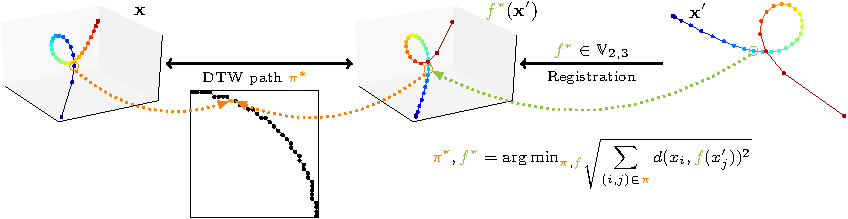
\includegraphics[width=\linewidth]{fig/dtw_gi_cropped}
    \caption{DTW-GI aligns time series by optimizing on temporal alignment
    (through Dynamic Time Warping) and feature space transformation (denoted
    $f$ here). Time series represented here are color-coded trajectories, whose
    starting (resp. end) point is depicted in blue (resp. red).}
    \label{fig:dtw-gi}
\end{figure}



\subsubsection{Optimization}

Optimization of the quantity in Equation \eqref{eq:dtwgi} can be performed
\emph{via} Block Coordinate Descent.
In a nutshell, the optimization process alternates between the following
two steps:

\begin{enumerate}
\item for a fixed $f$, the optimal alignment path $\pi$ is obtained through the
DTW algorithm;
\item for a fixed path $\pi$, the optimal map $f$ (when $\mathcal{F}$ is the
Stiefel manifold) is obtained through Singular Value Decomposition.
\end{enumerate}

Interestingly, this optimization strategy where we alternate between time
series alignment, \emph{i.e.} time correspondences between both time series, and
feature space transform optimization can be seen as a variant of the Iterative
Closest Point (ICP) method in image registration~\cite{CHEN1992145}, in
which  nearest neighbors are replaced by matches resulting from DTW alignment.

We also introduce soft counterparts following the definition of softDTW
from~\cite{cuturi2017soft}.
In this case, the optimization process consists of a gradient descent, and a
wider variety of
feature space transformation families can be considered.

\begin{figure}[t]
	\centering
	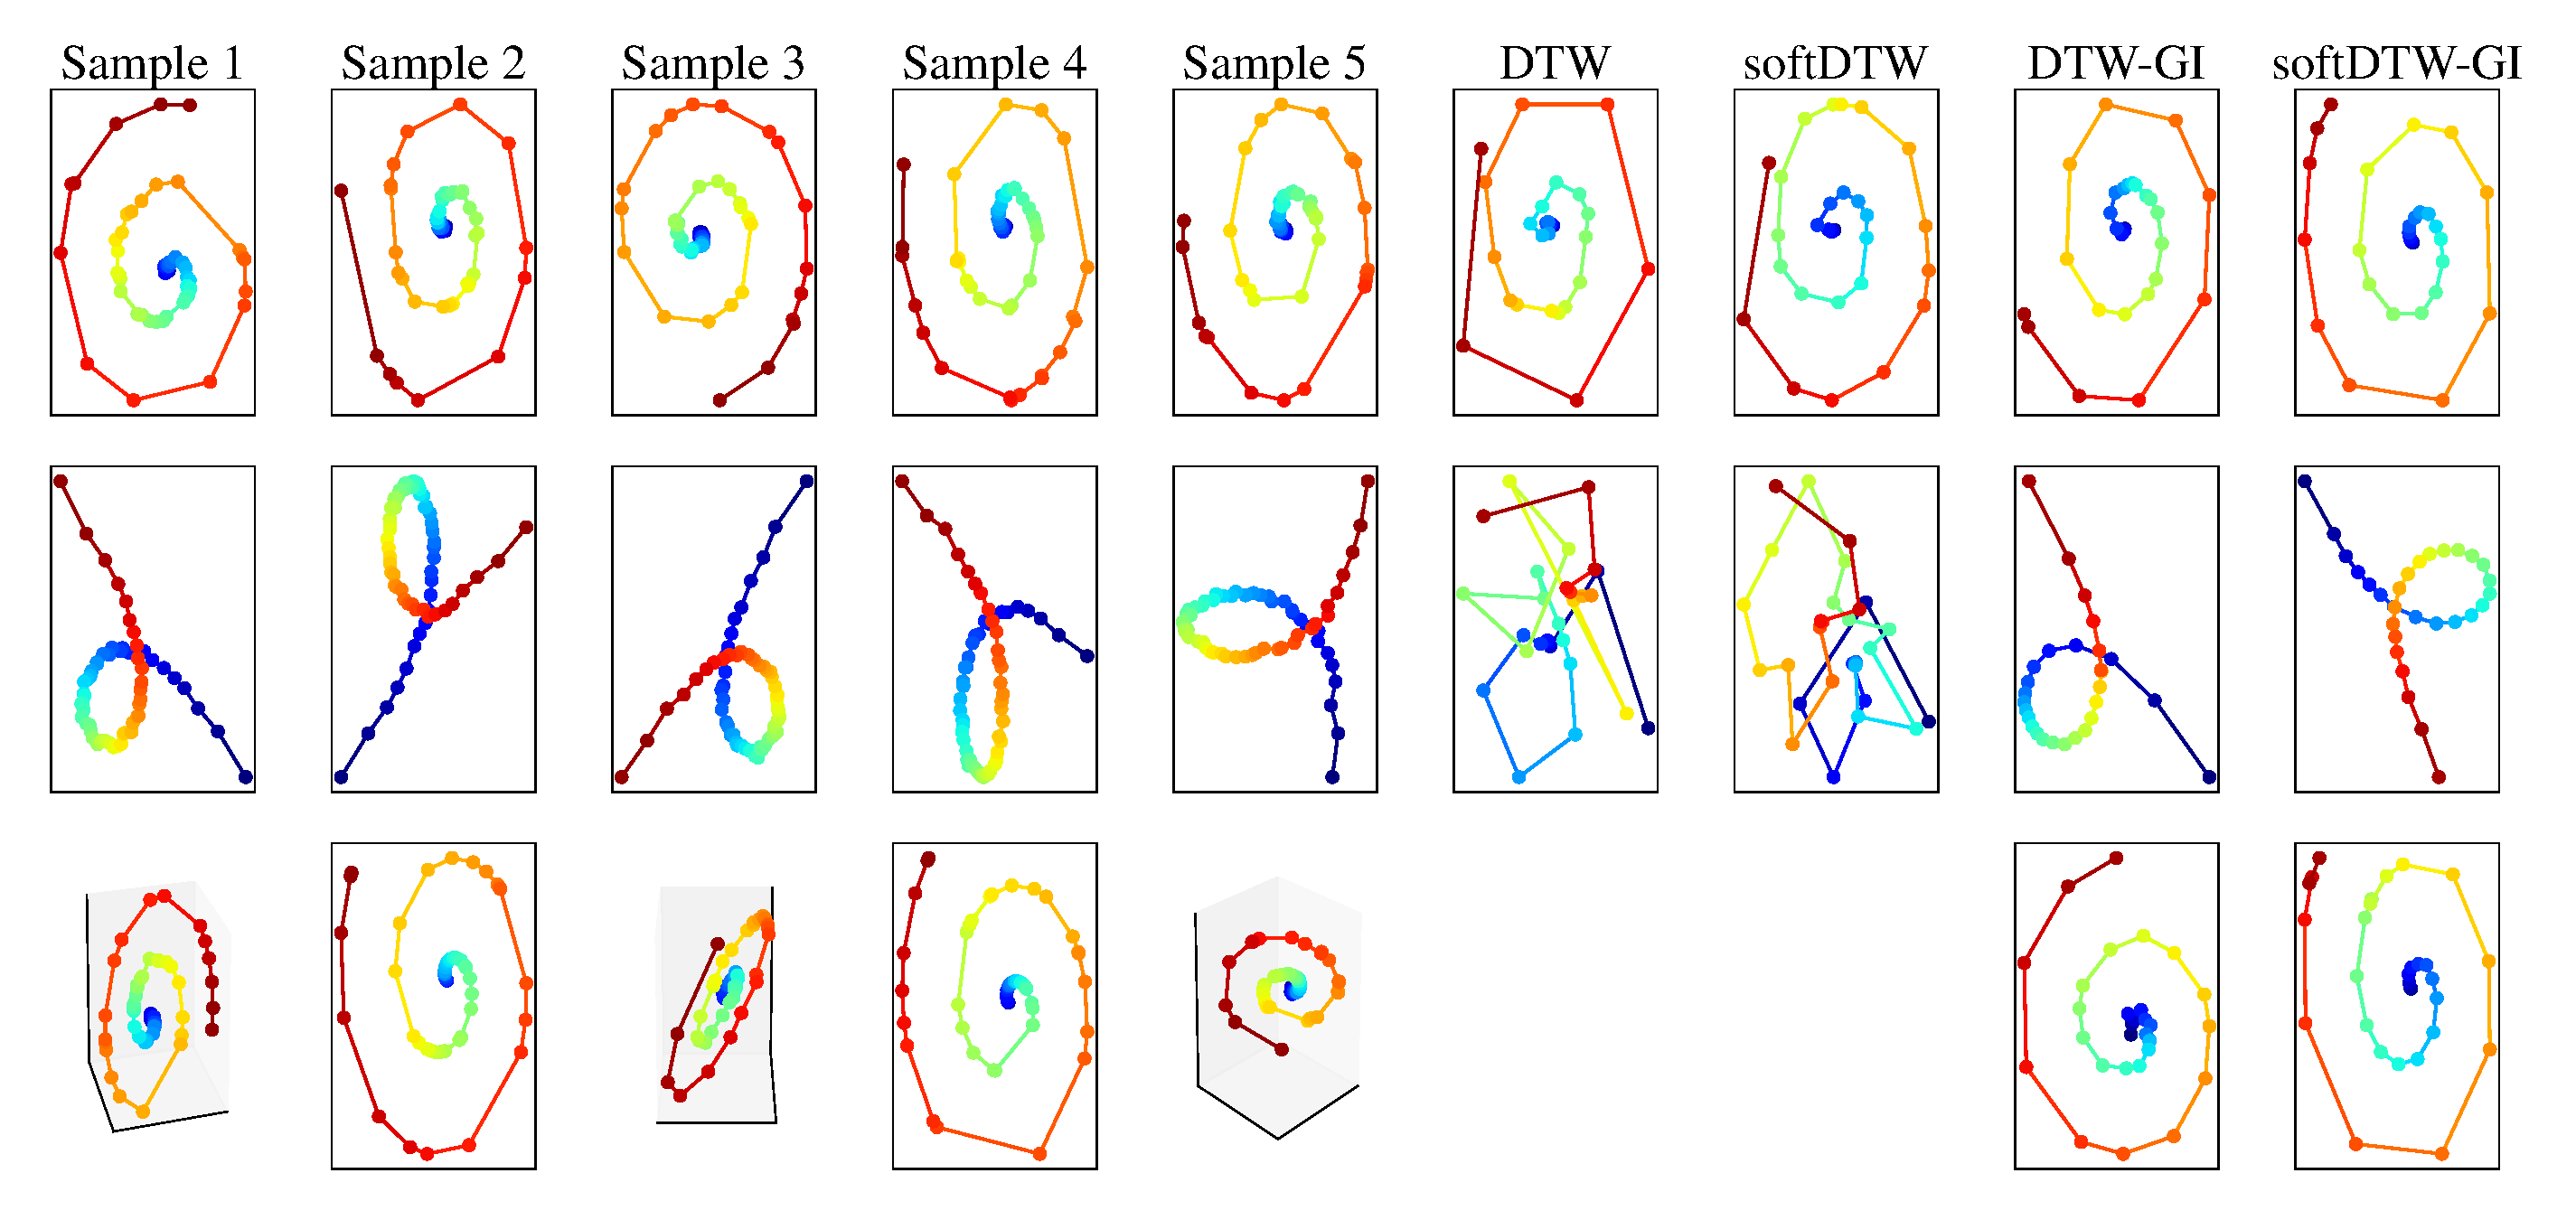
\includegraphics[width=\linewidth]{fig/barycenter_toys_allinone}
	\caption{
		Barycenter computation using (i) DTW and softDTW baseline approaches, (ii) their rotation-invariant counterparts DTW-GI and soft-DTW-GI.
		Each row correspond to a different dataset, and the latter one contains both 2d and 3d trajectories, hence cannot be tackled by any baseline method.
		Trajectories are color-coded from blue (beginning of the series) to red (end of the series).
		\label{fig:dtw_gi_bary}
	}
\end{figure}

To illustrate the interest of our approach,
Figure~\ref{fig:dtw_gi_bary} presents examples of barycenters obtained with
various DTW-based barycenter computation methods.
We validate the utility of these similarity measures on real world
datasets on the tasks of human motion prediction (where motion is captured under
different points of view) and cover song identification (where song similarity
is defined up to a key transposition).
In both these settings, we observe that joint optimization on feature space
transformation and temporal alignment improves over standard approaches that
consider these as two independent steps.
